\section{WiFi-Adapter testen}
Vor dem Aufsetzen des Tor-Proxys sollte zuerst überprüft werden, ob der angeschaffte WiFi-Adapter auf dem aufgespielten Betriebssystem lauffähig ist. Dazu steckt man den Adapter in den USB-Port und ruft nach kurzer Wartezeit folgendes Kommando auf:

\begin{lstlisting}
ifconfig -a
\end{lstlisting}

Wenn auf der erschienenen Ausgabe ein Eintrag für \textit{wlan0} zu sehen ist, kann mit der Einrichtung des Access Points begonnen werden.

\begin{figure}[H]
\centering
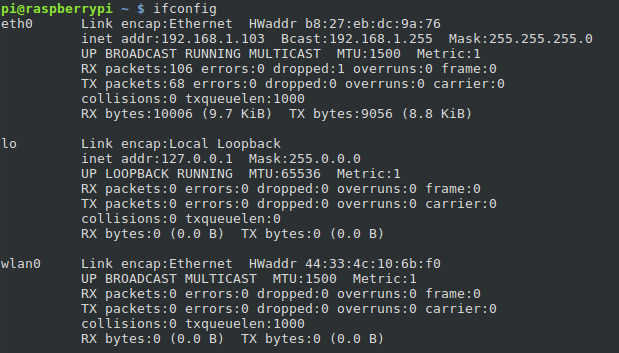
\includegraphics[scale=0.7]{images/ifconfig}
\caption{ifconfig - wlan0}
\end{figure}

\section{Access Point aufsetzen}
Mit dem eingesteckten Netzwerkkabel und dem per USB angeschlossenen WiFi-Adapter stehen nun zwei Netzwerk-Schnittstellen zur Verfügung. Das Netzwerkkabel hat die Aufgabe, den Raspberry Pi mit dem Internet zu verbinden. Der WiFi-Adapter hingegen soll so eingerichtet werden, dass er ein lokales WLAN (Wireless Local Area Network) aufzieht. Der Raspberry Pi fungiert somit als Wireless Access Point - auf deutsch so viel wie "kabelloser Zugangspunkt". Ein Access Point ermöglicht es Geräten wie Notebooks oder Smartphones, sich über ihn kabellos mit dem Internet zu verbinden. Neben der Software für den Access Point wird ein eigener DHCP-Server benögtigt. DHCP (Dynamic Host Configuration Protocol) ist ein Protokol, das die automatische Einbindung eines Computers in ein bestehendes Netzwerk ermöglicht. Der DHCP-Server sorgt also dafür, dass jeder Computer, der sich mit dem WLAN verbindet, eine valide IP-Adresse erhält und somit ein Teil des Netzes werden kann.
\\
Mit den folgenden befehlen werden die benötigten Softwarekomponenten installiert.
 
\begin{lstlisting}
apt-get install hostapd isc-dhcp-server
\end{lstlisting}

\subsection{DHCP-Server konfigurieren}
Damit der DHCP-Server auch richtig funktioniert, muss er zuerst konfiguriert werden.
Dazu öffnet man die Datei \textit{/etc/dhcp/dhcpd.conf} mit einem beliebigen Texteditor. In diesem Tutorial wird für diesen und alle nachfolgenden Fälle der vorinstallierte Texteditor \textit{nano} verwendet.
\\
Mit dem folgenden Kommando wird die Textdatei mit \textit{nano} geöffnet:

\begin{lstlisting}
nano /etc/dhcp/dhcpd.conf
\end{lstlisting}

Zuerst müssen die folgenden Zeilen gefunden und mittels einer vorangestellten Raute (\#) auskommentiert werden. Auskommentieren bedeutet, dass die Zeile ungültig und somit nicht mehr aktiv ist.

\begin{lstlisting}
option domain-name "example.org"
option domain-name-server ns1.example.org,ns2.example.org
\end{lstlisting}

Neu sieht das Ganze folgendermassen aus:

\begin{lstlisting}
#option domain-name "example.org"
#option domain-name-server ns1.example.org,ns2.example.org
\end{lstlisting}

Als Nächstes muss dem DHCP-Server mitgeteilt werden, dass er der offizielle DHCP-Server des zu erstellenden WLAN-Netzes ist. Einmal eingestellt vergibt er fortan valide IP-Adressen an jeden Computer, der dem Netz beitreten möchte.
\\
Dazu muss folgende Zeile einkommentiert - die vorangestellte Raute entfernt - werden:

\begin{lstlisting}
#authoritative;
\end{lstlisting}

Die Zeile sollte nun so aussehen:

\begin{lstlisting}
authoritative;
\end{lstlisting}

Das künftig vom WiFi-Adapter aufzuziehende WLAN muss einen eigenen Bereich zugewiesen bekommen, in dem es wirken kann.
\\
Dazu einfach die folgenden Zeilen ans Ende der Datei anfügen:

\begin{lstlisting}
subnet 192.168.66.0 netmask 255.255.255.0 {
  range 192.168.66.10 192.168.66.50;
  option broadcast-address 192.168.66.255;
  option routers 192.168.66.1;
  default-lease-time 600;
  max-lease-time 7200;
  option domain-name "local";
  option domain-name-servers 8.8.8.8, 8.8.4.4;
}
\end{lstlisting}

Der DHCP-Server ist fertig konfiguriert und muss an ein Netwerkinterface (Netzwerkschnittstelle) gebunden werden. Das gesuchte Netzwerkinterface ist in diesem Fall \textit{wlan0}, wie man schon zu beginn mittels \textit{ifconfig -a} herausgefunden hat.
In der Datei \textit{/etc/default/isc-dhcp-server} muss dazu bei der Einstellung \textit{INTERFACES} der Wert \textit{wlan0} eingetragen werden:

\begin{lstlisting}
INTERFACES="wlan0"
\end{lstlisting}

Dem Interface \textit{wlan0} kann jetzt eine fixe IP-Adresse vergeben werden. Es handelt sich dabei um jene Adresse, die bei der Konfiguration des DHCP-Server bei \textit{option routers} angegeben wurde - in diesem Fall also \textit{192.168.66.1}. 
\\
In der Datei \textit{/etc/network/interfaces} müssen zuerst folgende Zeilen auskommentiert werden:

\begin{lstlisting}
iface wlan0 inet manual
wpa-roam: /etc/etc/wpa_supplicant/wpa_supplicant.conf
iface default inet dhcp
\end{lstlisting}

Anschliessend fügt man folgende Zeilen hinzu:

\begin{lstlisting}
iface wlan0 inet static
  address 192.168.66.1
  netmask 255.255.255.0
\end{lstlisting}

\begin{figure}[H]
\centering
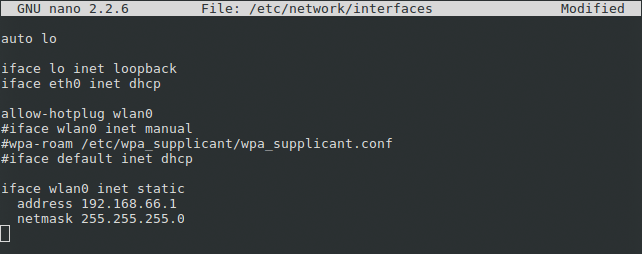
\includegraphics[scale=0.65]{images/network_interfaces.png}
\caption{konfigurierte interfaces-Datei}
\end{figure}

Das Interface \textit{wlan0} läuft zu diesem Zeitpunkt bereits. Um die eben getätigten Einstellungen sofort wirksam zu machen, muss noch folgendes Kommando abgesetzt werden:

\begin{lstlisting}
ifconfig wlan0 192.168.66.1
\end{lstlisting}

\subsection{Hostapd konfigurieren}
Nach dem DHCP-Server muss jetzt der Access Point konfiguriert werden. Die Konfigurationsdatei für \textit{hostapd} existiert aber noch nicht. Die neue Datei erstellt man mit:

\begin{lstlisting}
touch /etc/hostapd/hostapd.conf
\end{lstlisting}

Die Datei sollte jetzt erstellt sein und kann mit einem Texteditor geöffnet werden:

\begin{lstlisting}
nano /etc/hostapd/hostapd.conf
\end{lstlisting}

Folgende Zeilen müssen hinzugefügt werden:

\begin{lstlisting}
interface=wlan0
driver=rtl871xdrv
ssid=PiProxy
hw_mode=g
channel=6
macaddr_acl=0
auth_algs=1
ignore_broadcast_ssid=0
wpa=2
wpa_passphrase=Test1234
wpa_key_mgmt=WPA-PSK
wpa_pairwise=TKIP
rsn_pairwise=CCMP
\end{lstlisting}

Ein paar der obigen Werte kurz erklärt: 
\begin{itemize}
\item driver: Der Treiber-Name des Wifi-Adapters
\item ssid: Der Name des Netzes, wie man es nach aussen hin sieht
\item wpa\_passphrase: Passwort für den Zugang zum Netz
\end{itemize}

\textit{hostapd} kennt diese neue Konfiguration noch nicht. Um diese dem Programm bekanntzumachen, muss in der Datei \textit{/etc/default/hostapd} nach \textit{DAEMON\_CONF} gesucht und die Zeile wie folgt geändert werden:

\begin{lstlisting}
DAEMON_CONF="/etc/hostapd/hostapd.conf"
\end{lstlisting}

Der Raspberry Pi (Tor-Proxy) kann nun auf der einen Seite ein WLAN aufziehen und sich auf der anderen Seite mit dem Internet verbinden. Was jetzt noch fehlt ist die Verbindung dazwischen.

\subsection{NAT konfigurieren}
NAT (Network Address Translation) wird verwendet, um die mit dem WLAN verbundenen Geräte ins Internet weiterzuleiten. Der Datei \textit{/etc/sysctl.conf} muss dazu folgende Zeile angefügt werden:

\begin{lstlisting}
net.ipv4.ip_forward=1
\end{lstlisting}

Folgender Befehl macht die Einstellung umgehend aktiv:

\begin{lstlisting}
echo 1 > /proc/sys/net/ipv4/ip_forward
\end{lstlisting}

Zusätzlich muss die Firewall so eingestellt werden, dass NAT die eingerichtete Weiterleitung durchführen kann:

\begin{lstlisting}
iptables -t nat -A POSTROUTING -o eth0 -j MASQUERADE

iptables -A FORWARD -i eth0 -o wlan0 -m state --state RELATED,ESTABLISHED -j ACCEPT

iptables -A FORWARD -i wlan0 -o eth0 -j ACCEPT
\end{lstlisting}

Damit man diese Befehle nicht bei jedem Neustart des Raspberry Pi eingeben muss, können sie permanent gespeichert werden:

\begin{lstlisting}
iptables-save > /etc/iptables.ipv4.nat
echo "up iptables-restore < /etc/iptables.ipv4.nat" >> /etc/network/interfaces
\end{lstlisting}

\section{Erster Start des Access Points}
Der Access Point ist an diesem Punkt fast vollständig aufgesetzt. Um zu überprüfen, ob alles richtig gemacht wurde, muss man das Programm zusammen mit der Konfigurationsdatei aufrufen:
\begin{lstlisting}
/usr/sbin/hostapd /etc/hostapd/hostapd.conf
\end{lstlisting}

Entspricht die Ausgabe der unten Abgebildeten, waren die bisherigen Schritte erfolgreich und das nachfolgende Kapitel kann übersprungen werden.

\begin{figure}[H]
\centering
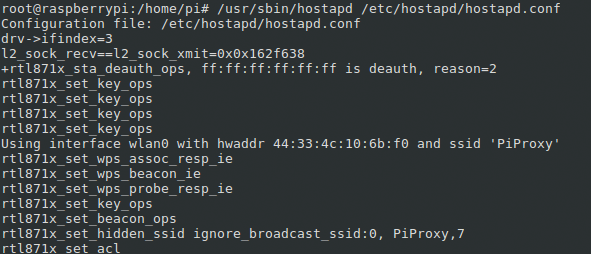
\includegraphics[scale=0.7]{images/hostapd_firststart}
\caption{hostapd- Ausgabe vom Erststart}
\end{figure}

\subsection{Fehlerbehandlung}
Tritt ein Fehler auf, liegt das möglicherweise an einer Inkompatibilität zwischen \textit{hostpad} und dem WiFi-Adapter bzw. dessen Treiber. Für den in diesem Tutorial verwendeten WiFi-Adapter kann das Problem gelöst werden, indem man \textit{hostapd} selber kompilliert. Dazu müssen mehrere Schritte befolgt werden.
\\
Achtung: Die Dateinamen und Verzeichnisse können sich je nach Fall von den hier Verwendeten unterscheiden und müssen dementsprechend angepasst werden.
\\
\\
Zuerst lädt man von der Hersteller-Seite den Linux-Treiber herunter. Dazu geht man auf \url{http://realtek.com} und navigiert zu \textit{Downloads > Communications Network ICs > Wireless LAN ICs > WLAN NIC > IEEE 802.11b/g/n Single-Chip > Software}. Dort lädt man den Linux-Treiber für den vom  WiFi-Adapter verwendeten Chipsatz herunter (hier RTL8192CU).
\\
Den heruntergeladenen Treiber (Zip-Datei) kopiert man auf einen USB-Stick und von dort in das Home-Verzeichnis des Raspberry Pi. Ist der USB-Stick am Pi angeschlossen, müssen dazu folgende Befehle abgesetzt werden:

\begin{lstlisting}
mount /dev/sda1 /mnt
cp /mnt/RTL8188C_8192C_USB_linux_v4.0.2_9000.20130911.zip /home/pi
umount /dev/sda1
\end{lstlisting} 

Anschliessend entpackt man die Zip-Datei:

\begin{lstlisting}
cd /home/pi
unzip RTL8188C_8192C_USB_linux_v4.0.2_9000.20130911.zip
\end{lstlisting}

Danach wechselt man in das richtige Verzeichnis und entpackt dort das Archiv, welches \textit{hostapd} enthält:

\begin{lstlisting}
cd wpa_supplicant_hostapd
tar -xzvf wpa_supplicant_hostapd-0.8_rtw_r7475.20130812.tar.gz
\end{lstlisting}

Danach wechselt man wiederum in das soeben entpackte Verzeichnis, wechselt in den Ordner namens \textit{hostapd} und startet den Kompiliervorgang:

\begin{lstlisting}
cd wpa_supplicant_hostapd-0.8_rtw_r7475.20130812/hostapd
make
\end{lstlisting}

Nach ein paar Minuten Wartezeit steht die frisch kompilierte, binäre Datei bereit. Diese wird in Zukunft die zu Beginn des Tutorials installierte Version ersetzen. Zuvor sollte man aber sicherheitshalber die Original-Datei sichern:

\begin{lstlisting}
mv /usr/sbin/hostapd /usr/sbin/hostapd.ORIG
\end{lstlisting}

Anschliessend kann man die neue \textit{hostapd}-Binärdatei kopieren:

\begin{lstlisting}
cp hostapd /usr/sbin	
\end{lstlisting}

Jetzt ist es an der Zeit, die ersten Schritte des Hauptkapitels \textit{Erster Start des Access Points} noch einmal auszuführen. Funktioniert es dieses Mal, kann mit dem nächsten Kapitel fortgefahren werden. Kommt es erneut zu Fehlern, sollten alle vorherigen Schritte genau überprüft und allenfalls die Internet-Community zu Rate gezogen werden.

\subsection{Verbindung herstellen zum Access Point}
Bevor man sich mit dem Access Point verbinden kann, müssen die beiden Komponenten \textit{hostapd} und \textit{isc-dhcp-server} gestartet werden:

\begin{lstlisting}
service hostapd start
service isc-dhcp-server start
\end{lstlisting}

Das WLAN sollte jetzt aktiv und für jedes WiFi-fähige Geräte erkennbar sein.

\begin{figure}[H]
\centering
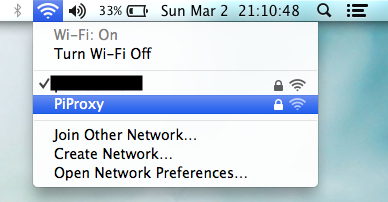
\includegraphics[scale=0.7]{images/accesspoint}
\caption{Der erstellte Access Point}
\end{figure}

\section{Daemons einrichten}
Beide Komponenten sollten als sogenannter \textit{Daemon} eingerichtet werden. Daemons sind Programme, die bei jedem Computerstart ebenfalls gestartet werden und fortan im Hintergrund laufen. Man will den Access Point schliesslich nicht jedes Mal manuell über die Konsole starten müssen. 

\begin{lstlisting}
update-rc.d hostapd enable 
update-rc.d isc-dhcp-server enable
\end{lstlisting}

Um die Daemons auf korrekte Funktionsweise zu überprüfen, muss der Tor-Proxy neu gestartet werden:

\begin{lstlisting}
shutdown -r now 
\end{lstlisting}

Ist der Computer wieder hochgefahren, fragt man die Stati der beiden Daemons ab:

\begin{lstlisting}
service hostapd status
service isc-dhcp-server status
\end{lstlisting}

Die Ausgabe sollte wie folgt aussehen: 

\begin{figure}[H]
\centering
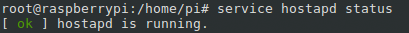
\includegraphics[scale=0.7]{images/hostapd_status}
\caption{Status Access Point}
\end{figure}

\begin{figure}[H]
\centering
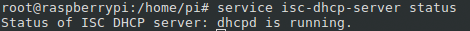
\includegraphics[scale=0.7]{images/dhcp_status}
\caption{Status DHCP-Server}
\end{figure}

Verhält sich der Access Point nicht wie gewünscht oder läuft gar nicht erst, empfiehlt es sich, alle vorherigen Schritte noch einmal zu studieren und die Konfigurationen zu überprüfen. Für schwer zu lösende Probleme kann man sich auch immer an die Internet-Gemeinschaft wenden. Waren alle bisherigen Schritte erfolgreich, kann jetzt damit begonnen werden, den eigentlichen Tor-Proxy aufzusetzen.

\section{Tor aufsetzen}
An dieser Stelle ist es möglich, sich mittels Access Point mit dem Internet zu verbinden und loszusurfen. Das Ziel ist es aber, die Verbindung ins Internet über das Tor-Netzwerk zu leiten, um ein gewisses Mass an Anonymität zu gewährleisten. Dafür muss als erstes die entsprechende Softwarekomponente installiert werden. Tor kann man - wie die zuvor verwendeten Programme auch - über die Paketverwaltung installieren:

\begin{lstlisting}
apt-get install tor
\end{lstlisting}

Nach der Installation muss Tor natürlich noch richtig konfiguriert werden: 

\begin{lstlisting}
nano /etc/tor/torrc
\end{lstlisting} 

Direkt nach dem einleitenden Kommentarblock müssen folgende Zeilen hinzugefügt werden:

\begin{lstlisting}
Log notice file /var/log/tor/notices.log
VirtualAddrNetwork 10.192.0.0/10
AutomapHostsSuffixes .onion,.exit
AutomapHostsOnResolve 1
TransPort 9040
TransListenAddress 192.168.66.1
DNSPort 53
DNSListenAddress 192.168.66.1
\end{lstlisting}

Die Datei sollte nun folgendermassen aussehen: 

\begin{figure}[H]
\centering
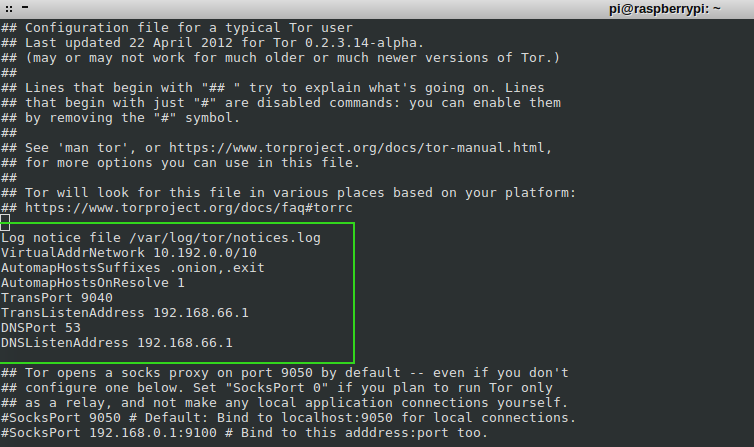
\includegraphics[scale=0.6]{images/torrc}
\caption{torrc-Datei}
\end{figure}
 	
Der Firewall muss jetzt noch beigebracht werden, dass jegliche Kommunikation vom WLAN ins Internet über das Tor-Netzwerk geleitet werden soll:

\begin{lstlisting}
iptables -F

iptables -t nat -F

iptables -t nat -A PREROUTING -i wlan0 -p tcp --dport 22 -j REDIRECT --to-ports 22

iptables -t nat -A PREROUTING -i wlan0 -p udp --dport 53 -j REDIRECT --to-ports 53

iptables -t nat -A PREROUTING -i wlan0 -p tcp --syn -j REDIRECT --to-ports 9040

iptables-save > /etc/iptables.ipv4.nat
\end{lstlisting}

\subsection{Protokollierung aktivieren}
In der \textit{torrc}-Konfigurationsdatei wurde bei \textit{Log notice file} eine Datei angegeben, die in Zukunft alle Logs enthält. Mit \textit{Logs} sind Protokolleinträge gemeint, die von der Tor-Software erstellt werden und Auskunft über den Status und allfällige Probleme geben. Diese Datei muss erstellt und mit den entsprechenden Rechten versehen werden:

\begin{lstlisting}
touch /var/log/tor/notices.log
chown debian-tor /var/log/tor/notices.log
chmod 644 /var/log/tor/notices.log
\end{lstlisting}

Nun muss man den Tor-Service neu starten, damit die vorgenommenen Einstellungen aktiv werden:

\begin{lstlisting}
service tor restart
\end{lstlisting}

Um zu prüfen, ob Tor erfolgreich gestartet werden konnte, kann man folgenden Befehl ausführen:

\begin{lstlisting}
service tor status
\end{lstlisting}

Die Ausgaben sollten wie die unten Abgebildeten aussehen.

\begin{figure}[H]
\centering
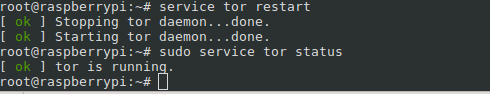
\includegraphics[scale=0.7]{images/tor_service}
\caption{Tor - Neustart und Status}
\end{figure}

Auch Tor soll bei jedem Start des Systems automatisch laufen. Um Tor als Daemon zu konfigurieren, muss man analog zu vorhin folgenden Befehl absetzen:

\begin{lstlisting}
update-rc.d tor enable
\end{lstlisting}

Der Access Point und Tor sind an diesem Punkt fertig installiert und eingerichtet. Gratuliere! Jetzt fehlt nur noch ein abschliessender Test, um sicherzustellen, dass alles so funktioniert, wie es soll.

\section{IP-Adresse verifizieren}
Mittels \url{http://wieistmeineip.ch} kann die IP-Adresse ermittelt werden, mit der man sich im Internet bewegt. Diese wird einem normalerweise vom Provider zugeteilt und ändert sich eher selten. Mit einem funktionierenden Tor-Setup ändert sich dieses Verhalten jedoch. Da je Anfrage ins Internet drei verschiedene Tor-Server passiert, ändert sich die Absender-IP-Adresse des Paketes jedes Mal. Die angefragte Internetseite sieht somit nie die IP-Adresse, die einem vom Provider zugeteilt wurde, sondern immer die des zuletzt passierten Tor-Servers - auch Exit-Node genannt. Um die korrekte Funktionsweise des Tor-Proxys zu verifizieren, muss man lediglich von einem Computer im normalen Netz und einem Gerät, das mittels Tor-Proxy mit dem Internet verbunden is, die Seite \textit{wieistmeineip} aufrufen. Die IP-Adressen und auch die sonstigen angezeigten Informationen dürfen sich bei einem funktionierenden Tor-Proxy nicht decken.

\begin{figure}[H]
\centering
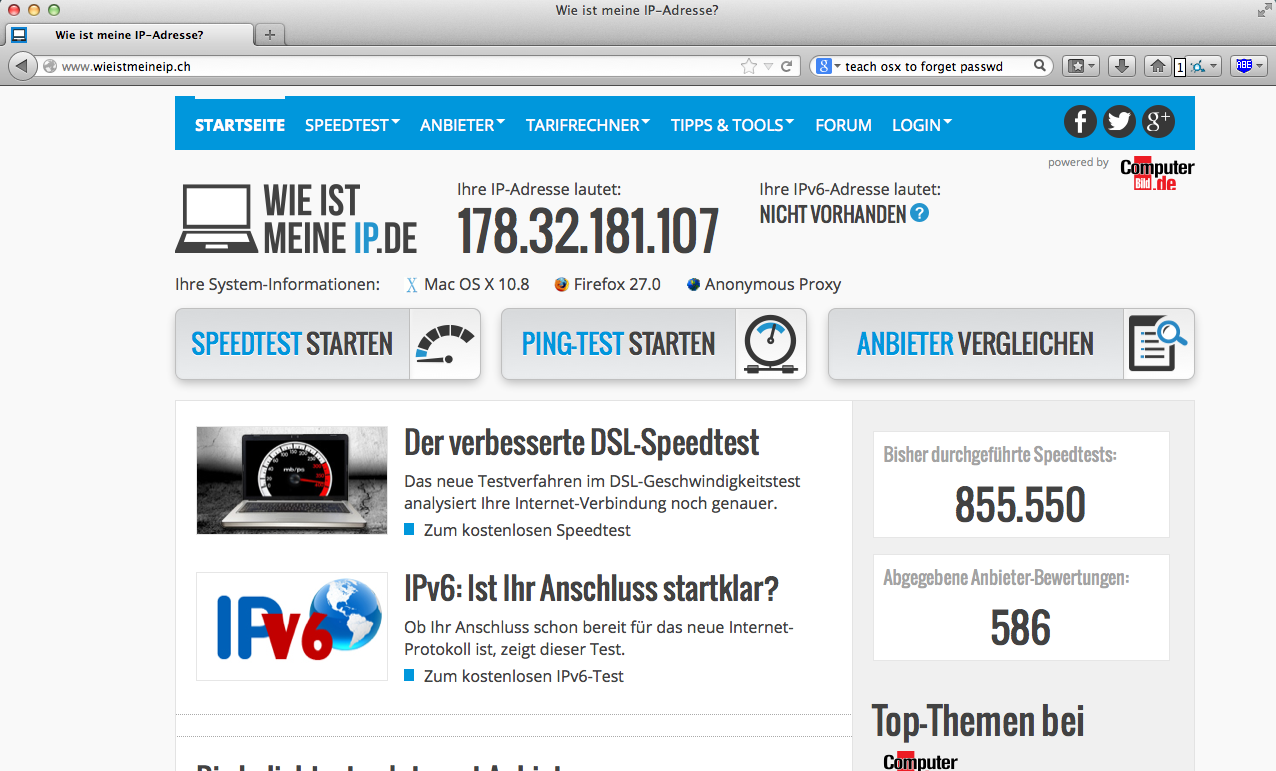
\includegraphics[scale=0.4]{images/wieistmeineip}
\caption{wieistmeineip.ch mit funktionierendem Tor-Proxy}
\end{figure}

Zusätzlich dazu kann die Seite \url{https://check.torproject.org/} besucht werden. Diese zeigt einem an, ob man mittels Tor im Internet unterwegs ist und liefert gleich noch ein paar hilfreiche Links.

\begin{figure}[H]
\centering
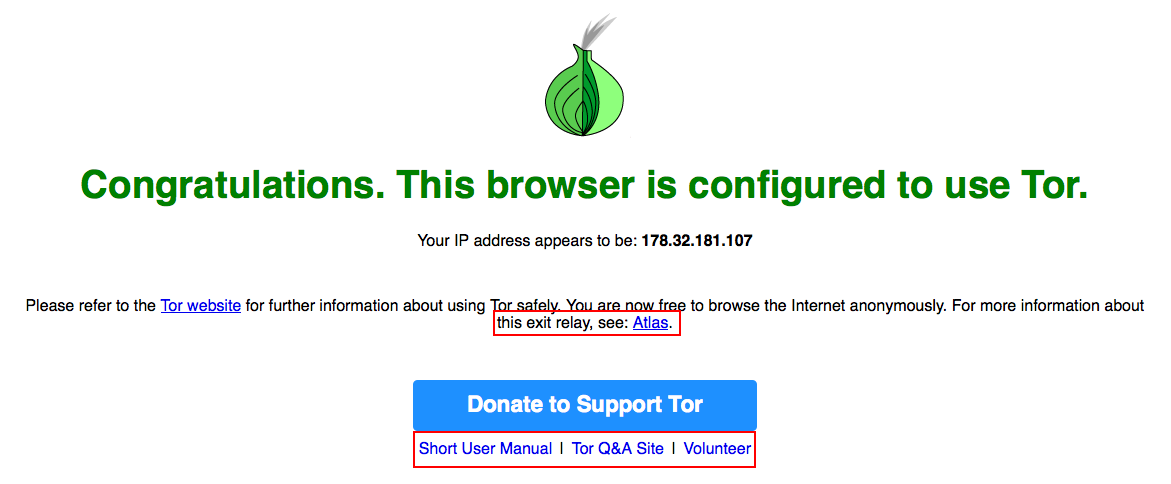
\includegraphics[scale=0.4]{images/torcheck}
\caption{Tor-Check}
\end{figure}

\section{Exit-Nodes konfigurieren}
Will man den Tor-Proxy bzw. deren Verwendung sicherer gestalten, lohnt es sich, die zugelassenen Exit-Nodes festzulegen. Der letzte Tor-Server auf dem Weg zum Ziel ist bekanntlich der Exit-Node. Er übernimmt das versendete Paket vom vorherigen Tor-Server, entpackt es und leitet es schliesslich an die Zieladresse weiter. Entpacken bedeutet, dass er je nach verwendetem Protokoll - http oder https - alle Details des Pakets einsehen kann. Da jeder einen solchen Exit-Node betreiben kann - gut gesinnte Privatpersonen oder Organisationen, Geheimdienste oder sonstige Kriminelle - kann man nie genau wissen, wer jetzt einen sogenannten \textit{Bad-Exit-Node} betreibt. Glücklicherweise kann dieses Risiko minimiert werden. In der Tor-Konfigurationsdatei \textit{torrc} kann man festlegen, welche Exit-Nodes verwendet werden sollen und/oder nur Exit-Nodes aus gewissen Ländern zulassen. Es gibt diverse Organisationen und Verbünde, die solche Tor-Exit-Nodes betreiben und zum Gebrauch anbieten. Eine davon ist die Swiss Privacy Foundation: \url{http://privacyfoundation.ch/}.
\\
Um die Exit-Nodes einzuschränken bzw. nach seinen persönlichen Wünschen zu selektieren, gibts es zwei Möglichkeiten, die sich mitunter sogar kombinieren lassen: 

\begin{enumerate}
\item Angabe des \textit{Fingerprints} (eindeutige ID) eines spezifischen Exit-Nodes
\item Angabe eines Ländercodes, wodurch nur Exit-Nodes von diesem Land verwendet werden
\end{enumerate}

Die Einstellungen werden in der \textit{torrc}-Konfigurationsdatei vorgenommen. Diese  muss man zuerst mittels Texteditor öffnen:

\begin{lstlisting}
nano /etc/tor/torrc
\end{lstlisting}

Die folgenden Zeilen werden nach \textit{DNSListenAddress 192.168.66.1} angefügt:

\begin{lstlisting}
StrictNodes 1
ExitNodes Fingerprint1,Fingerprint2,{Laendercode1},{Laendercode2},{Laendercode3}
\end{lstlisting}

Beim Fingerprint handelt es sich um eine lange Kombination aus Zahlen und Buchstaben mit einem vorangestellten \$-Zeichen. Beispielsweise hat ein von der \textit{Swiss Privacy Foundation} bereitgestellter Exit-Node den Fingerprint \$944224E9413705EEAFCBAC98BF57C475EB1960C5.
Zwischen den geschweiften Klammern kann ein Ländercode angegeben werden. Für Exit-Nodes aus der Schweiz müsste man \{ch\} verwenden. Man kann dabei so viele Länder angeben wie man will. 
\\
Wichtig ist, dass alle angegebenen Optionen (Ländercodes und Fingerprints) stets mittels Komma getrennt werden und keine Leerzeichen dazwischenstehen.
\\
\\
Ein weiteres Beispiel soll ein bisschen Klarheit schaffen:

\begin{lstlisting}
ExitNodes $944224E9413705EEAFCBAC98BF57C475EB1960C5,{de},{at}
\end{lstlisting}

Mit dieser Einstellung werden nur deutsche und österreichische Exit-Nodes verwendet inklusive einem zu Bginn einzeln definierten Exit-Node.

\section{Abschluss}
Tor bietet noch viele andere Möglichkeiten, den Dienst den eigenen Ansprüchen anzupassen und sicherer zu machen. Details zu den unterschiedlichen Konfigurationen und Modi findet man hier: \url{https://www.torproject.org/docs/tor-manual.html.en}. Die Seite ist zur Zeit leider nur auf Englisch verfügbar. Es gibt zudem gewisse Verhaltensregeln, die für einen sinnvollen und sicheren Gebrauch von Tor befolgt werden sollten: 

\begin{itemize}
\item Verwendung vom verschlüsselten https-Protokoll an Stelle von http wenn immer möglich!
\item Keine Soziale Netzwerke besuchen!
\item Sich nirgends einloggen oder registrieren - zumindest nicht mit Daten, die Rückschlüsse auf die Identität zulassen!
\item Cookies weitgehend deaktivieren, JavaScript deaktivieren
\end{itemize}

Achtung: Ein falscher und verantwortungsloser Gebrauch von Tor birgt mehr Gefahren, als wenn man ganz auf den Dienst verzichten würde. Deshalb sollte man sich vor Gebrauch von Tor gut über die verschiedenen Funktionen und Risiken informieren. Im Internet findet man allerhand an Material und Informationen, um sattelfest auf dem Gebiet zu werden. Ist man einmal sattelfest, steht einem sinnvollen Gebrauch von Tor nichts mehr im Weg. Viel Spass! 